\chapter{Wyniki}
\label{cha:wyniki}

\section{N gier 3-osobowych niezależnych}
\label{sec:N3nzal}

\paragraph{Równania standardowe}
\label{sec:r_stan}

%---------------------------------------------------------------------------------------------------------------------------------------------------------
\paragraph{Równania replikatorów}
\label{sec:r_repl}

%---------------------------------------------------------------------------------------------------------------------------------------------------------
\section{N gier 3-osobowych zależnych}
\label{sec:N3zal}
\begin{wrapfigure}{rh}{0.5\textwidth}
    \centering
    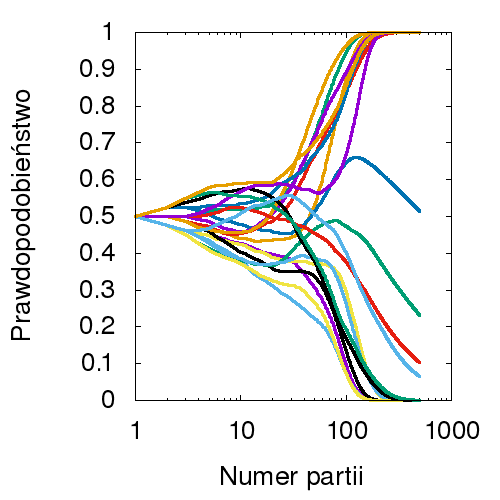
\includegraphics[width=0.5\textwidth]{pict/wyniki/g500p20}   
    \caption{500 gier, 20 graczy}
	\label{fig:podst} 
\end{wrapfigure}

Chciałbym teraz przeanalizować wyniki jednej z symulacji \ref{fig:podst}. Jak już wcześniej zaobserwowaliśmy równania replikatorów dają dużo mniejszą dynamikę decyzji graczy.

Peleton graczy tworzy stabilne koalicje około 300 partii które nie są w stanie ulec zmianie. Pozostałe przypadki tworzą niestabilne koalicje, które zmieniają się w czasie. Najlepszym tego przykładem jest gracz który początkowo gra w kierunku swojego prawego sąsiada, a później zapewne przez jego niechęć po kilku fluktuacjach zaczyna drastycznie zmieniać partnera swojej gry - zaznaczonych kolorem fioletowym. Czynnik losowy graczy utrudnia grę tylko z jednym wybranym partnerem, dlatego jak widzimy podczas pierwszych 50 gier dochodzi do dużej liczby zmian zachowań graczy. Szczególnie widoczne jest to w pierwszych 50 partiach, gdzie gracze dopiero szacują zachowanie sąsiadów. W kolejnych 50 partiach gracze zachowują się coraz bardziej liniowo, gdyż błąd przewidywanego i realnego prawdopodobieństwa przeciwnika spada. Nie wchodzący w stałą koalicja mogą należeć do łańcucha graczy niezdecydowanych lub jednostek znajdujących się pomiędzy dwoma silnymi koalicjami które nie dają szansy na przyłączenie się do żadnej. Wartym zauważenia jest fakt że ostatnia zmiana monotoniczności funkcji zachodzi dopiero około 300 gry.

Rozpatrzmy teraz dużo dłuższą grę w której zaangażowanych jest więcej graczy, co może pokazać nam przypadki szczególne. Na rysunku widzimy że większość zawodników osiąga stabilne koalicję przed grą 1000. Widzimy grupkę kilku graczy którzy pomimo tak dużej ilości gier nie byli w stanie zawiązać trwałych koalicji.

CHECK
Mogło to wynikać z dwóch faktów. Po pierwsze mogli znaleźć się między graczami znajdującymi się w trwały w sojuszach którzy nie byli zainteresowani wchodzeniem w nowe. Drugą przyczyną może być nieznajomość prawdziwego prawdopodobieństwa podejmowania decyzji przez sąsiadów które jest tylko wartością znaną z rozgrywki różnica pomiędzy faktycznym prawdopodobieństwem gry sąsiada a tym co reprezentował w rozgrywce może się znacząco różnić wpływając na Mylna ocenę prawdopodobieństwa gry zawodników i mogących ustalić 1a stabilnej koalicji rysunek 3 pokazuje przypadek w którym dwóch silnych policjantów nie nie jest zainteresowanych wejście w sojusz z osamotnionych zawodnikiem


%\lipsum[1-15]

\begin{figure}
	\label{niechciani}
	\subfloat[10000 gier, 200 graczy]{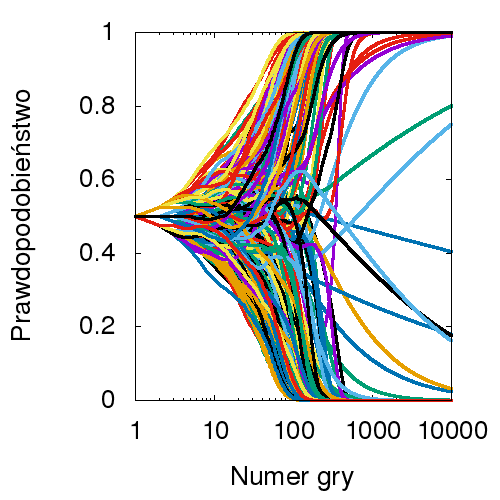
\includegraphics[width=.5\textwidth]{pict/wyniki/g10000p200}}
	\subfloat[KOMENT!!!!]{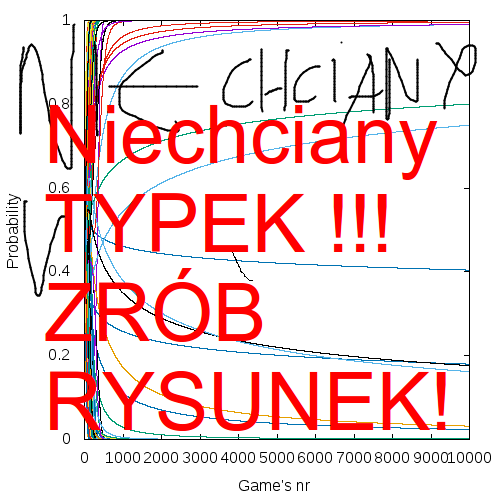
\includegraphics[width=.5\textwidth]{pict/wyniki/niechciany}}
\caption{Długa gra}
\end{figure}